\section{INTRODUCTION}
This chapter describes the collected data and analysis of the data. Expected results and actual results are discussed here and the deviation of the actual results from expected results are shown. The improvements that could be done  to minimize deviation from the expected is also discussed within this chapter. Further improvements that can be done for the research and how those improvements can be done are also discussed.

\section{ANALYSIS OF DATA}
Data collection has been done for 07 times per location (selected $1m^2$ area)to collect Wi-Fi RSSI values for each location by using developed android application. Each collected data has been analyzed separately and finally all data had been analyzed with respect to each location. The data analyzation will be discussed here after.

\newpage
\subsection{ACCESS POINT 01 DATA ANALYSIS}  
\begin{center}
	\begin{figure*}[h]	
		\centering
		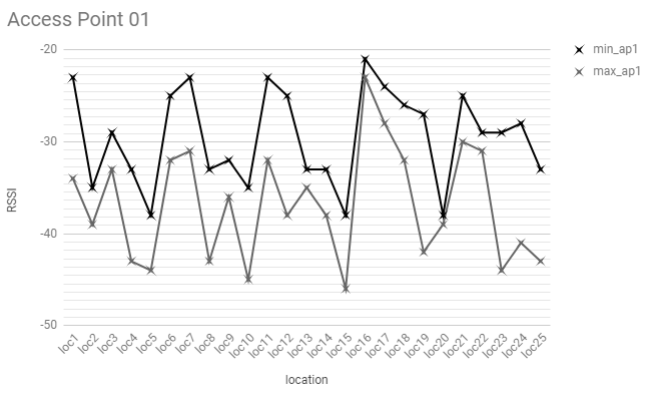
\includegraphics[width=1\textwidth]{ap1.png}
		\caption{Access Point 01 data analysis}
	\end{figure*}
\end{center} 

This line chart shows the Wi-Fi RSSI range of access point 01 (Wi-Fi enterprise support access point which directly communicates with FreeRADIUS server). There are two graphs in the chart which clearly shows minimum RSSI values of each location and maximum RSSI value of each location. It can be identified that the difference between maximum and minimum RSSI value of each location is around 10 dB's.

\newpage
\subsection{ACCESS POINT 02 DATA ANALYSIS}  
\begin{center}
	\begin{figure*}[h]	
		\centering
		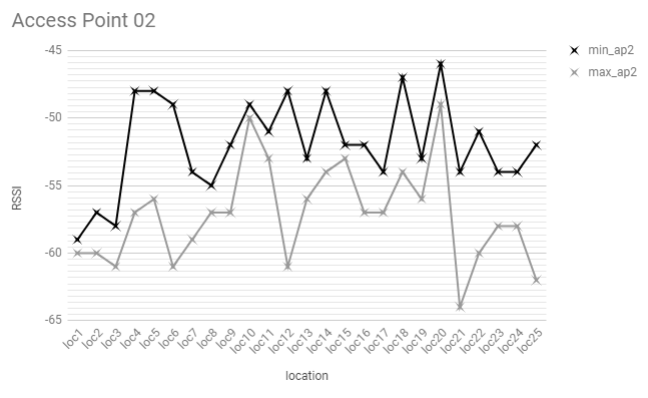
\includegraphics[width=1\textwidth]{ap2.png}
		\caption{Access Point 02 data analysis}
	\end{figure*}
\end{center} 

This line chart shows the Wi-Fi RSSI range of access point 02. There are two graphs in the chart which clearly shows minimum RSSI values of each location and maximum RSSI value of each location. Not like the previous access point, this access point is located outside the research area which has physical obstacles. It seems that the signal strength of this access point is fluctuate significantly.

\newpage
\subsection{ACCESS POINT 03 DATA ANALYSIS}  
\begin{center}
	\begin{figure*}[h]	
		\centering
		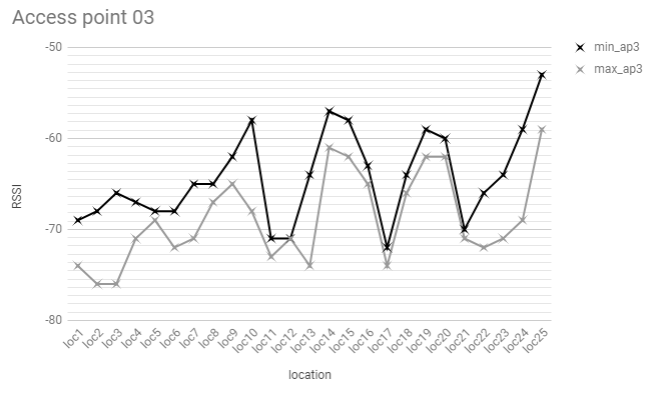
\includegraphics[width=1\textwidth]{ap3.png}
		\caption{Access Point 03 data analysis}
	\end{figure*}
\end{center} 

This line chart shows the Wi-Fi RSSI range of access point 03. There are two graphs in the chart which clearly shows minimum RSSI values of each location and maximum RSSI value of each location. This access point is also located outside the research area which has physical obstacles. But as an average, this access point is far away from the research area. Therefore, the signal strength of this access point is much weaker than the previous two access points.

\newpage 
\subsection{ALL ACCESS POINT DATA ANALYSIS}  
\begin{center}
	\begin{figure*}[h]	
		\centering
		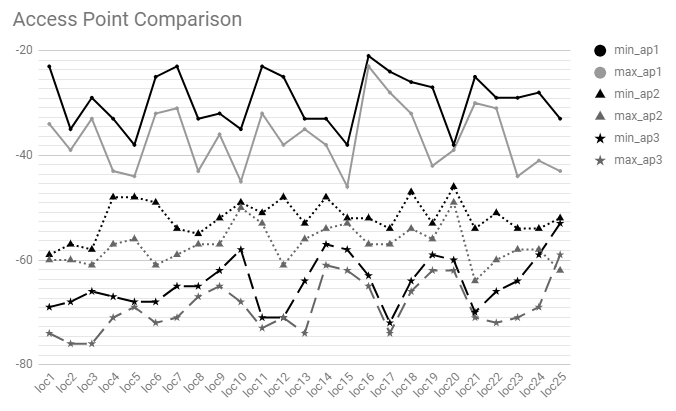
\includegraphics[width=1\textwidth]{total_comparison.png}
		\caption{Access Point data analysis}
	\end{figure*}
\end{center} 

All three(03) access point RSSI values are compared here. Each access point is marked by a separate symbol.

\newpage
\subsection{LIVE USER ACCESS DATA ANALYSIS}

In this phase, user live access data has been collected for the access attempts of 140. 125 readings have been taken within the research area where the location fingerprinting has been done. The rest of the readings were taken by accessing the system from outside of the research area. The testing of the system has been carried out with uncontrollable noisy of additional Wi-Fi signals.

\begin{figure*}[h]
	\centering
	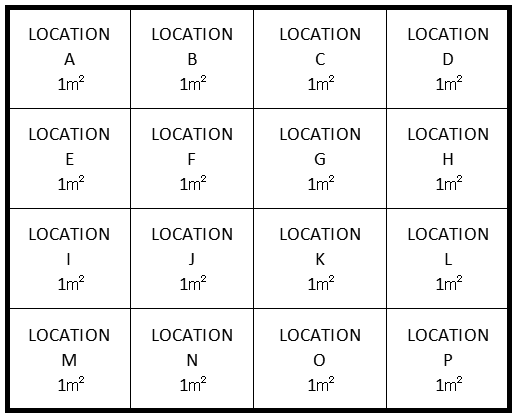
\includegraphics[width=0.4\textwidth]{fp.png}
	\caption{Wi-Fi fingerprinting area}
\end{figure*}
Refer appendix \ref{LOCATION ONE TEST} for each location test results.

\paragraph{}
By analyzing the test results, it is possible to identify that some location results are significantly deviated from the expected results. There could be several reasons for the deviation.

\subsubsection{OVERALL TEST RESULT}
\begin{table}[H]
	\centering
	\label{OVERALL TEST RESULT}
	\begin{tabular}{lllll}
		NO OF LOCATIONS& :&  25&    \\
		SUM OF PASS RATE& :& 1980&  \\
		SUM OF FAIL RATE& :& 520&   \\\\
		AVERAGE PASS RATE& :& $\frac{1980}{25}$&   \\\\
		AVERAGE FAIL RATE& :& $\frac{520}{25}$&  \\\\
		OVERALL PASS RATE& :& \verb|79.20%|&   
	\end{tabular}
	\caption{Overall Test Results}
\end{table} 


\section{FACTORS EFFECTING TO WIRELESS NETWORK SIGNAL}
It is well known that wireless networks use electromagnetic waves(radio waves) for the communication. Even though electromagnetic waves do not require any medium for propagation, there are many factors that could be affected to the performance of the Wi-Fi network. Some of those cannot be avoided and measures have to be taken to minimize the negative effects which are affecting on the performance. The rest of the factors can be completely resolved by either through a good network planning or equipment upgrading.\cite{signal_probs}
\begin{itemize}
	\item Network range and distance between devices
	
	\begin{figure*}[h]	
		\centering
		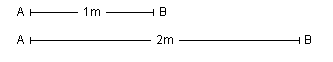
\includegraphics[width=0.4\textwidth]{distance.png}
		\caption{Signal strength with distance}
	\end{figure*}
	
	\subitem  Due to the wireless signal propagation within wide areas when they travel further, the signals become weaker. Inverse Square Law \eqref{eq:1} denotes this relationship between signal strength and the distance.
	
	\item Physical interference
	\subitem There is a possibility of penetrating Wi-Fi signals through solid objects such as buildings, walls, hills or even people. The more obstacles between signal generator and receiver, the more impact on signal strength. With lower frequency of the signal, there is a high impact on the signal strength. And also with higher frequency, the reflection capabilities get increased. However in some cases, reflecting may work better rather than trying to send it directly.
	
	\item Network usage
	\subitem Wireless networks allow more than one user to communicate over the channel simultaneously. That means the network resources are utilized by many users and when more devices are connected to the access point, it easily comes to the threshold level and this makes a reduction in performance.
	
	\item Wireless network interference
	\subitem Since wireless networks are common, more wireless transmissions are being sent through the open air and those signals could be operated at similar frequencies. It is well known and proved that the waves operating at similar frequencies can cause an interference with each other and the resultant signal may completely different from the generated signal. Other wireless technologies such as microwave, mobile phone signals that operate within the same range could be affected to the signals as well. But most of the devices are designed to minimize such effects as much as possible by the design, but still the effects are present with an acceptable level.
	
	\item Environmental characteristics
	\subitem Physically,concrete wall obstacles are the biggest constraint of wireless signals. The materials used in the walls may have different levels of effects as well. And also the humidity in air also effects the signal strength, negatively. The moisture in the air makes it more difficult for the signal to be sent efficiently.\cite{humidity_issue} Other than that, any object which is located between signal transmitter and receiver can absorb some sort of energy of the signal, which may result a negative impact on the signal strength within the area.
\end{itemize}  


\section{FURTHER IMPROVEMENTS}
The suggested approach is expected to pass more than \verb|90%| test cases but the actual pass rate of the total test cases is less than expected rate. Because of this, more improvements are required to gain the pass rate of test cases as expected.

\begin{itemize}
	\item Collect more location data to improve accuracy of the location fingerprint database
		\subitem The research has been carried out with seven(07) rounds of data collection sets. More collected location data can minimize the Wi-Fi RSSI value reading errors.
		
	\item Collect data with different conditions.
		\subitem Data can be collected in both calm and noisy environmental conditions. But collecting data should be done carefully as noisy and bad environmental conditions can badly affect to the Wi-Fi RSSI values, Which may result in accepting users those who are coming from the outside of the allowed location.
		
	\item Harden the RADIUS server to avoid possible vulnerabilities.
		\subitem The system completely depends on location fingerprint database. Therefore separate, dedicated user should be used for RADIUS server rather than super user.
		
	\item Encrypt data objects from Android mobile application to RADIUS server.
		\subitem Data object (JSON object) is a plain text format. It could be vulnerable for sniffing attacks. It should use a proper encryption method to encrypt data.
		
	\item Add a separate database user for MySQL database (Location fingerprint database).
		\subitem It is better to use a separate user for database transactions rather than using super user with a complex password. This separate user should be able to perform only the following operations.
			\subsubitem Read data
			\subsubitem Write data
			\subsubitem Update data
		 
	\item Build self-learned location fingerprint database
		\subitem Collect data of the Wi-Fi signal strengths at real time by using android application to build self-learned Wi-Fi fingerprint database. Authentication failures could be minimized by this such as mistakes of initial training database errors.
		
	\item Minimize human errors when collecting initial data collection
		\subitem Human errors are common in most of the systems and it is difficult to minimize. The same person could be used to collect data, to minimize human errors which can be happened when collecting initial Wi-Fi signal data.
\end{itemize}